% IF YOU CAN SEE THIS GO CONTRIBUTE >:( nah fuck u but thanks

\documentclass[letterpaper, 8pt]{extarticle}
\usepackage{amssymb,amsmath,amsthm,amsfonts}
\usepackage{multicol,multirow}
\usepackage{calc}
\usepackage{ifthen}
\usepackage[landscape]{geometry}
\usepackage[colorlinks=true,citecolor=blue,linkcolor=blue]{hyperref}
\usepackage{booktabs}
\usepackage{ulem}
\usepackage{enumitem}
\usepackage{tabulary}
\usepackage{graphicx}
\usepackage{siunitx}
\usepackage{tikz}
\usepackage{derivative}
\usepackage{svg}
\usepackage{listings}
\usepackage{setspace} 
\usepackage{listings}
\usepackage{xcolor}
\usepackage{courier}
\usepackage{amsthm}
\newtheorem{theorem}{Theorem}

\setstretch{0.1}

\ifthenelse{\lengthtest { \paperwidth = 11in}}
    { \geometry{top=.25in,left=.25in,right=.25in,bottom=.35in} }
	{\ifthenelse{ \lengthtest{ \paperwidth = 297mm}}
		{\geometry{top=1cm,left=1cm,right=1cm,bottom=1cm} }
		{\geometry{top=1cm,left=1cm,right=1cm,bottom=1cm} }
	}

\newenvironment{Figure}
  {\par\medskip\noindent\minipage}
  {\endminipage\par\medskip}

\pagestyle{empty}
\makeatletter
\renewcommand{\section}{\@startsection{section}{1}{0mm}%
                                {-1ex plus -.5ex minus -.2ex}%
                                {0.5ex plus .2ex}%x
                                {\normalfont\normalsize\bfseries}}
\renewcommand{\subsection}{\@startsection{subsection}{2}{0mm}%
                                {-1explus -.5ex minus -.2ex}%
                                {0.5ex plus .2ex}%
                                {\normalfont\small\bfseries}}
\renewcommand{\subsubsection}{\@startsection{subsubsection}{3}{0mm}%
                                {-1ex plus -.5ex minus -.2ex}%
                                {1ex plus .2ex}%
                                {\normalfont\tiny\bfseries}}
\makeatother
\setcounter{secnumdepth}{0}
\setlength{\parindent}{0pt}
\setlength{\parskip}{0pt plus 0.5ex}
% -----------------------------------------------------------------------
% \tymin=37pt
% \tymax=\maxdimen

% Custom siunitx defs
\DeclareSIUnit\noop{\relax}

\NewDocumentCommand\prefixvalue{m}{%
\qty[prefix-mode=extract-exponent,print-unity-mantissa=false]{1}{#1\noop}
}

% Shorthand definitions
\newcommand{\To}{\Rightarrow}
\newcommand\ttt\texttt

% prettier CTL/LTL
\DeclareMathOperator{\X}{X}
\DeclareMathOperator{\F}{F}
\DeclareMathOperator{\G}{G}
\DeclareMathOperator{\U}{U}
\DeclareMathOperator{\W}{W}
\DeclareMathOperator{\R}{R}
\DeclareMathOperator{\A}{A}
\DeclareMathOperator{\E}{E}
\DeclareMathOperator{\AX}{AX}
\DeclareMathOperator{\EX}{EX}
\DeclareMathOperator{\AG}{AG}
\DeclareMathOperator{\EG}{EG}
\DeclareMathOperator{\AU}{AU}
\DeclareMathOperator{\EU}{EU}
\DeclareMathOperator{\AF}{AF}
\DeclareMathOperator{\EF}{EF}

% condense itemize & enumerate
\let\olditemize=\itemize \let\endolditemize=\enditemize \renewenvironment{itemize}{\olditemize \itemsep0em}{\endolditemize}
\let\oldenumerate=\enumerate \let\endoldenumerate=\endenumerate \renewenvironment{enumerate}{\oldenumerate \itemsep0em}{\endoldenumerate}
\setlist[itemize]{noitemsep, topsep=0pt, leftmargin=*}
\setlist[enumerate]{noitemsep, topsep=0pt, leftmargin=*}

\title{2SD3}

\begin{document}

\raggedright
\tiny

\lstdefinelanguage{FSP}{
  morekeywords={
    const, range,
    when,
    forall,
    if, then, else,
    property, progress,
    fluent, assert, exists,
  },
  morecomment=[l]{//},
  morecomment=[s]{/*}{*/},
}
\lstset{
tabsize = 1, %% set tab space width
showstringspaces = false, %% prevent space marking in strings, string is defined as the text that is generally printed directly to the console
basicstyle = \tiny \ttfamily , %% set listing font and size
breaklines = true, %% enable line breaking
numberstyle = \tiny,
postbreak = \mbox{\textcolor{red}{$\hookrightarrow$}\space},
language = FSP
}

\begin{center}
  {\textbf{2SD3 Final v0.2 -- The Triumph of Bureaucracy and Vocal Minority: You Shall (Not) Pass Edition}} \\
\end{center}
\setlength{\premulticols}{1pt}
\setlength{\postmulticols}{1pt}
\setlength{\multicolsep}{1pt}
\setlength{\columnsep}{2pt}
\begin{multicols*}{5}
% vvvvv contribution notice - remove me later vvvvv
{
\color{red}
If you're reading this, please contribute!
}

REMINDER! This is a template! The cheat sheet maintainer (.json) \textit{intentionally} leaves extra space for you to add your own notes! If something's missing, add it yourself! (and if it's important enough please contribute!)
% ^^^^^ contribution notice - remove me later ^^^^^
% \section{planning (remove me later)}
% \begin{itemize}
%     \item FSP
%     \item LTS
%     \item Elem. Petri
%     \item Concurrent Composition
%     \item Bisimulation
%     \item Labeling \& Hiding
%     % \item Structure Diagrams
%     \item Mutexes
%     \item Monitors and Buffers
%     \item Semaphores, Limits, and Extensions
%     \item Deadlock
%     \item P/T Nets
%     \item Coloured Petri Nets
%     \item Safety and Liveness
%     \item Model Based Design (literally don't remember anything from this)
%     % \item Message Passing (ch 14 not on it)
%     \item LTL and CTL (and CTL*)
%     \item Model Checking
%     \item Dynamic Systems
%     % \item Timed Systems (no longer on exam)
    
%     % invariants? 
% \end{itemize}

\section{FSP}
\subsection{Syntax}
\begin{lstlisting}
// instance prefixing - a:P
SWITCH = (on -> off -> SWITCH).
||TWO_SWITCH = (a:SWITCH || b:SWITCH).

// relabeling - /{new1/old1, new2/old2, ...}.
CLIENT = (call -> wait -> continue -> CLIENT).
SERVER = (request -> service -> reply -> SERVER).
||CLIENT_SERVER = (CLIENT||SERVER)/{call/request,reply/wait}.

// process prefixing (mutex) - {a1, ..., ax} :: P
RESOURCE = (acquire -> release -> RESOURCE).
USER = (acquire -> user -> release -> USER).
||RESOURCE_SHARE = (a:USER || b:USER || {a, b}::RESOURCE).
// RESOURCE is a single shared instance between the two USERs

// for loop syntax
|| SWITCHES (N = 3) = (forall [i:1..N] s[i]:SWITCH)
// or alternatively
range Seats = 1..3
|| SEATS=(seat[i:1..3]:SEAT).

// hiding operator - \{a1, ..., ax}
// interface operator - @{a1, ..., ax}
// these two do the same thing
USER = (acquire -> use -> release -> USER)\{use}.
USER = (acquire -> use -> release -> USER)@{acquire, release}.

// syntax for progress
progress P = {a1, ..., an}

// syntax for high priority
||C = (P||Q)<<{a1, ..., an}.
// syntax for low priority
||C = (P||Q)>>{a1, ..., an}.

// simulating a boolean
const False = 0
const True  = 1
range Bool  = 0..1
\end{lstlisting}

Maker-user example
\begin{lstlisting}
MAKER = (make -> ready -> MAKER).
USER  = (ready -> user -> USER).
||MAKER_USER = (MAKER || USER).
\end{lstlisting}

Garden example (maybe move this to a diff section later)
\begin{lstlisting}
const N = 4
range T = 0..N
set VarAlpha = {value.{read[T],write[T]}}

VAR      = VAR[0],
VAR[u:T] = (read[u]   ->VAR[u] 
           |write[v:T]->VAR[v]).

TURNSTILE = (go    -> RUN),
RUN       = (arrive-> INCREMENT
            |end   -> TURNSTILE),
INCREMENT = (value.read[x:T]
            ->value.write[x+1]->RUN)
            +VarAlpha.

DISPLAY =(value.read[T]->DISPLAY)+{value.write[T]}.

||GARDEN = (east:TURNSTILE || west:TURNSTILE || display:DISPLAY
           || {east,west,display}::value:VAR)
            /{go /{east,west}.go,
              end/{east,west}.end}.
\end{lstlisting}

\section{LTS}
% TODO: This can probably be deleted, seems pretty trivial
% Maybe replace with crucial examples?
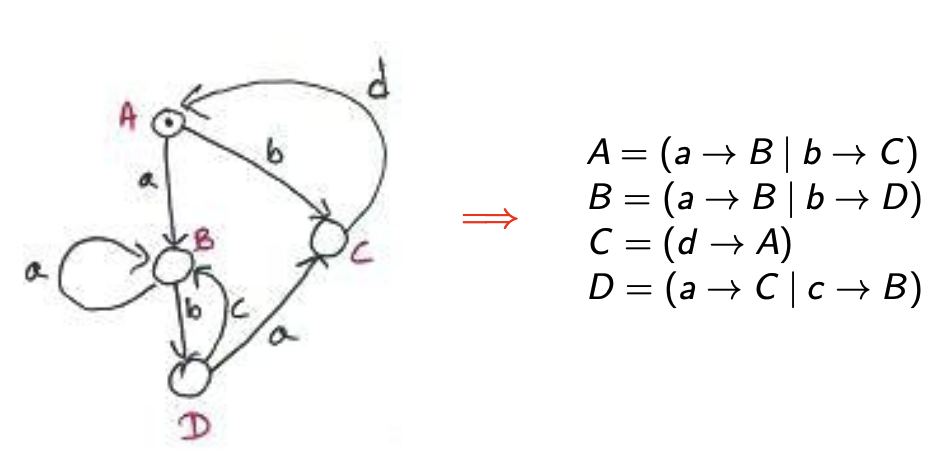
\includegraphics[width=\linewidth]{COMPSCI-2SD3/lts-example.png}

\section{Petri Nets}

\subsection{Reachability Graphs}
% TODO: this image is really small and probably won't print well
% if we have time, refactor it...
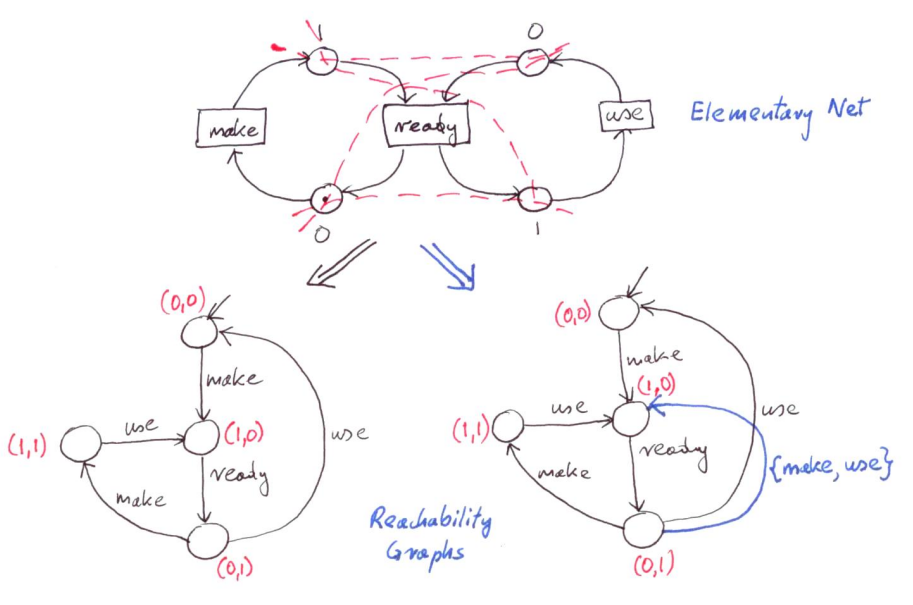
\includegraphics[width=\linewidth]{COMPSCI-2SD3/reachability_graph.png}

\section{Hiding/Labeling}
\textbf{relabeling:} (PROCESS)/$\{newlabel1/oldlabel1, ... , newlabeln/oldlabeln\}$\\
\textbf{interface:} (PROCESS)@$\{a1 . . . ax\}$ hides all actions except a1 . . . ax\\
\textbf{hiding:} (PROCESS) \textbackslash  $\{a1...an\}$ hides actions a1...an\\

$\{a1, . . . , ax\}$ :: P replaces every action label n in the alphabet
of P with the labels a1.n, ... , ax.n. Thus, every transition
(n → X) in the definition of P is replaced with the transitions
$(\{a1.n, . . . , ax.n\} \xrightarrow{} X)$

\section{Bisimulation}
\textbf{State Bisimilarity} -- $p \approx q$ iff whatever action executed at $p$ can also be executed at $q$, and vice versa.

\textbf{LTS Bisimilarity} -- $P \approx Q$ iff each state $p_t$, reachable from the initial state by a trace $t$ in $P$ is bisimilar to an appropriate state $q_t$ that is reachable from the initial state by the same trace $t$ in $Q$.

% \section{Structure Diagrams}
% \begin{center}
%     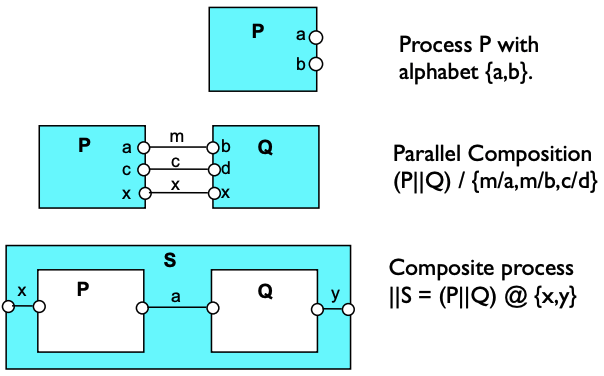
\includegraphics[width=\linewidth]{COMPSCI-2SD3/sd.png}
%     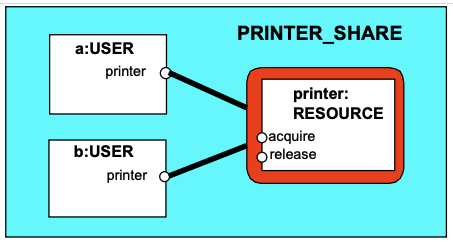
\includegraphics[width=.7\linewidth]{COMPSCI-2SD3/sd-printer.png}
% \end{center}
% \begin{lstlisting}
% RESOURCE = (acquire -> release -> RESOURCE).
% USER =     (printer.acquire->use->printer.release->USER)\{use}.

% ||PRINTER_SHARE
%     = (a:USER||b:USER||{a,b}::printer:RESOURCE).
% \end{lstlisting}

\section{Mutual Exclusion}
Arbitrary interleaving of read and write actions leads to \textbf{interference}.
Interference bugs are difficult to locate.
We use \textbf{mutual exclusion} to only give one process access to the shared resource at a time.

\begin{lstlisting}
LOCK = (acquire->release->LOCK).
U1 = (acquire -> use -> release -> U1).
U2 = (acquire -> use -> release -> U2).
||SYSTEM = (u1:U1||u2:U2||{u1,u2}::LOCK).
\end{lstlisting}
Above allows for lock$\xrightarrow{}$use$\xrightarrow{}$release for either user but only one of them at a time.

\section{Monitors and Semaphores}
\textbf{Monitor} -- A threadsafe class where each function is wrapped by a mutex. Essentially, only one process may access the class at a time. Entirely syntactic sugar.
\textbf{Semaphore} -- Essentially a mutex with a queue of processes

\begin{lstlisting}
down(s):    if s > 0 then
                decrement s
            else
                block execution of calling process
up(s):      if processes blocked on s then
                awaken one of them
            else
                increment s
\end{lstlisting}

\begin{lstlisting}
const Max = 3
range Int = 0..Max

SEMAPHORE(N=0) = SEMA[N],
SEMA[v:Int]    = (up->SEMA[v+1]
                 |when(v>0) down->SEMA[v-1]
                 ).

LOOP = (mutex.down -> critical -> mutex.up -> LOOP).

||SEMADEMO = (p[1..3]:LOOP || {p[1..3]}::mutex:SEMAPHORE(1)).
\end{lstlisting}
\section{Bounded Buffer}
A buffer with a fixed number of slots
\begin{lstlisting}
BUFFER(N=5) = COUNT[0],
COUNT[i:0..N]
    = (when (i<N) put->COUNT[i+1]
      |when (i>0) get->COUNT[i-1]
      ).
PRODUCER = (put->PRODUCER).
CONSUMER = (get->CONSUMER).

||BOUNDEDBUFFER = (PRODUCER||BUFFER(5)||CONSUMER).
\end{lstlisting}
\subsection{Nested Monitor Problem}
\section{P/T nets}
Each place in a P/T net can hold multiple tokens. Each transition has a weight, w, associated with it. If it is an input transition, firing takes w tokens from the input place. If its an output transition, firing adds w tokens to the output place. An action can only be fired if enough input tokens are present in all input places.
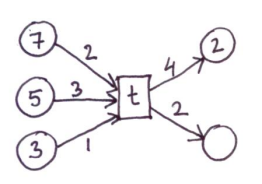
\includegraphics[width=.7\linewidth]{COMPSCI-2SD3/ptnet.png}
\section{Deadlocks}
\subsection{Dining Philosophers Problem}
Simple minded construction:
\begin{lstlisting}
FORK = (get -> put -> FORK).
PHIL = (think -> right.get -> left.get -> eat -> right.put -> left.put -> PHIL).
||DINERS(N = 5) = forall[i : 1..N] (phil[i] : PHIL || {phil[i].right, phil[(i % 5) + 1].left} :: FORK
\end{lstlisting}

\textbf{Solution 1} -- Add asymmetry into the composition, where 1, 3, 5 always perform `left.get -> right.get',
while 2, 4 always perform `right.get -> left.get'.
\begin{lstlisting}
PHIL = (when(i=1|i=3|i=5) think -> left.get -> right.get -> eat -> left.put -> right.put -> PHIL
       |when(i=2|i=4) think -> right.get -> left.get -> eat -> right.put -> left.put -> PHIL).
\end{lstlisting}

\textbf{Solution 2} -- Use a butler to prevent more than 4 philosophers from sitting at the table.
\begin{lstlisting}
PHIL = (think -> sitdown -> right.get -> left.get -> eat -> right.put -> left.put -> getup -> PHIL).
BUTLER(K=4) = COUNT[0],
COUNT[i:1..4] = (when(i<K) sitdown -> COUNT[i+1] | getup -> COUNT[i-1]).
||DINERS(N=5) ...
||{phil[i:1..N]}::BUTLER(K=4)).
\end{lstlisting}

\textbf{Solution 3} -- Use Simultaneity
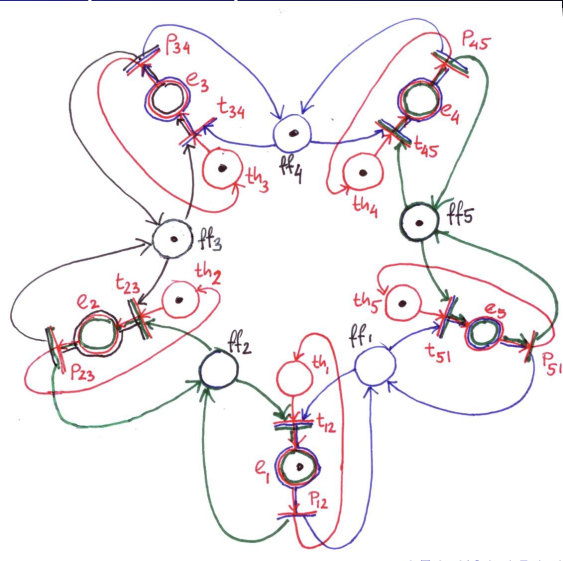
\includegraphics[width=\linewidth]{COMPSCI-2SD3/phil-sim.png}
Only fire a transition if both forks are available

\section{Coloured Petri Nets}
``Colours'' are simply types of tokens that are passed around the petri net
Paths to transitions are either labeled with variables or functions that transform one of the input variables into the object to remove from a state.

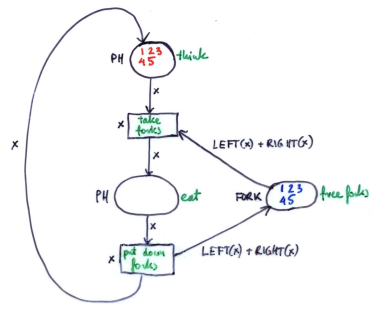
\includegraphics[width=\linewidth]{COMPSCI-2SD3/diners-cpn.png}
\begin{lstlisting}
colour PH = with ph1 | ph2 | ph3 | ph4 | ph5
colour Fork = with f1 | f2 | f3 | f4 | f5
LEFT : PH -> FORK, RIGHT : PH -> FORK
var x : PH
fun LEFT x = case of ph1 => f2 | ph2 => f3 | ph3 => f4 | ph4 => f5 | ph5 => f1
fun RIGHT x = case of ph1 => f1 | ph2 => f2 | ph3 => f3 | ph4 => f4 | ph5 => f5
\end{lstlisting}

\section{Semaphores and Extensions}
\subsection{Dijkstra's Semaphore Operations}
\textbf{C(s)} -- initial value of a semaphore variable $s$
\textbf{ndown(s)} -- number of times down(s) was executed
\textbf{nup(s)} -- number of times up(s) was executed
\textbf{npdown(s)} -- number of times down(s) was passed

Then we define down and up:\\
\textbf{down(s)}: ndown(s) = ndown(s)+1:
if ndown(s) <= nup(s) + C(s) then npdown(s) = npdown(s) + 1;\\
\textbf{up(s)}: if ndown(s) > nup(s) + C(s)
then npdown(s) = npdown(s) + 1; nup(s) = nup(s)+1;
\begin{theorem}
npdown(s) = min(ndown(s), C(s) + nup(s))
\end{theorem}

\subsection{Multidimensional Semaphores of Agerwala}
\textbf{edown($s1, \dots, s_n, s_{n+1}, \dots, s_{n+m}$}:
if for all $i, 1 \leq i \leq n, s_i > 0$ and for all $j, 1 \leq j \leq m, S_{n+j} = 0$
then for all $i, 1 \leq i \leq n, s_i = s_i - 1$
else block execution of calling processes

\textbf{eup($s_1, s_2, \dots, s_n$}:
if processes blocked on ($s_1, \dots, s_n$)
then awaken al of them
else for all $i, i \leq i \leq n, s_i = s_i + 1$

\subsection{Inhibitor Nets}
Add a circle to the transition side of an arc to make it an inhibitor arc
Now the transition can only be fired if the places connected by inhibitor arcs are empty.

\subsection{Smokers' Problem}
3 Smokers each have an unlimited type of either tobacco, cigarette paper, matches.
2 ingredients are placed on the table, the smoker with the third ingredient needed should pick up the ingredients, make a cigarette, and smoke it.
Next set of ingredients won't be placed until smoking is completed.

\subsubsection{Simple-minded Solution}
\begin{lstlisting}
SMOKER_T=( get_paper -> get_match->roll_cigarrette -> smoke_cigarrette -> SMOKER_T).
SMOKER_P=( get_tobacco -> get_match->roll_cigarrette -> smoke_cigarrette -> SMOKER_P).
SMOKER_M=( get_tobacco -> get_paper->roll_cigarrette -> smoke_cigarrette -> SMOKER_M).

TOBACCO = ( delivered -> picked -> TOBACCO ).
PAPER = ( delivered -> picked -> PAPER ).
MATCH = ( delivered -> picked -> MATCH ).

AGENT_T = (can_deliver -> deliver_paper -> deliver_match -> AGENT_T ).
AGENT_P = (can_deliver -> deliver_match -> deliver_tobacco -> AGENT_P ).
AGENT_M = (can_deliver -> deliver_tobacco -> deliver_paper -> AGENT_M ).

RULE = (can_deliver -> smoking_completed -> RULE ).

||SMOKERS = (s_t:SMOKER_T || s_p:SMOKER_P || s_m:SMOKER_M ).
||RESOURCES = ({s_m,s_p}::TOBACCO || {s_t,s_m}::PAPER || {s_t,s_p}::MATCH ).

||AGENT_RULE = ({s_m,s_p,s_t}::RULE || {s_m,s_p}::AGENT_T || {s_m,s_t}::AGENT_P ||
{s_t,s_p}::AGENT_M ).

||CIG_SMOKERS = (SMOKERS || RESOURCES || AGENT_RULE)/
{s_t.get_paper/s_t.picked,
 s_m.get_paper/s_m.picked,
 s_p.get_paper/s_p.picked,
 s_t.deliver_paper/s_t.delivered,
 s_m.deliver_paper/s_m.delivered,
 s_p.deliver_paper/s_p.delivered,
 s_t.smoking_completed/s_t.smoke_cigarrette,
 s_m.smoking_completed/s_m.smoke_cigarrette,
 s_p.smoking_completed/s_p.smoke_cigarrette}.
\end{lstlisting}

\subsubsection{Property (safety)}
\begin{lstlisting}
property CORRECT_PICKUP =
(s_t.get_paper->s_t.get_match->CORRECT_PICKUP
|s_p.get_tobacco->s_p.get_match->CORRECT_PICKUP
|s_m.get_tobacco->s_m.get_paper->CORRECT_PICKUP).
\end{lstlisting}

\subsubsection{Ask first, do later}
\begin{lstlisting}
SMOKER_T=( no_tobacco -> get_paper -> get_match->roll_cigarrette ->
smoke_cigarrette -> SMOKER_T)
SMOKER_P=( no_paper -> get_tobacco -> get_match->roll_cigarrette ->
smoke_cigarrette -> SMOKER_P)
SMOKER_M=( no_match -> get_tobacco -> get_paper->roll_cigarrette ->
smoke_cigarrette -> SMOKER_T)
TOBACCO = ( delivered -> picked -> TOBACCO )
PAPER = ( delivered -> picked -> PAPER )
MATCH = ( delivered -> picked -> MATCH )
AGENT_T = (can_deliver -> no_tobacco ->deliver_paper->deliver_match->AGENT_T)
AGENT_P = (can_deliver -> no_paper -> deliver_match->deliver_tobacco->AGENT_P)
AGENT_M = (can_deliver -> no_match -> deliver_tobacco->deliver_paper->AGENT_M)
RULE = (can_deliver -> smoking_completed -> RULE )

SMOKERS = s_t:SMOKER_T || s_p:SMOKER_P || s_m:SMOKER_M
RESOURCES = {s_m,s_p}::TOBACCO || {s_t,s_m}::PAPER || {s_t,s_p}::MATCH
AGENT_RULE = {s_m,s_p,s_t}::RULE || {s_m,s_p}::AGENT_T || {s_m,s_t}::AGENT_P || {s_t,s_p}::AGENT_M

CIG_SMOKERS = (SMOKERS || RESOURCES || AGENT_RULE)/
{s_t.get_paper/s_t.picked,
 s_m.get_paper/s_m.picked,
 s_p.get_paper/s_p.picked,
 s_t.deliver_paper/s_t.delivered,
 s_m.deliver_paper/s_m.delivered,
 s_p.deliver_paper/s_p.delivered,
 s_t.smoking_completed/s_t.smoke_cigarrette,
 s_m.smoking_completed/s_m.smoke_cigarrette,
 s_p.smoking_completed/s_p.smoke_cigarrette}.
\end{lstlisting}

\section{Safety and Liveness}
\textbf{Safety} -- asserts that nothing bad happens

\textbf{Safety Property} $P$ -- defines a process that asserts any trace including the actions in the alphabet of $P$ is accepted by $P$, otherwise they are transitions to the ERROR state, safety checks are compositional hence they should be composed with the appropriate (sub)system

\textbf{Liveness} -- asserts that something good eventually happens

\textbf{Progress Property} -- asserts that it is always the case that a particular action is eventually executed, opposite of starvation, progress checks are not compositional hence they should be conducted after safety checks

\textbf{Starvation} -- situation in which an action is never executed

\textbf{Terminal Set of States} -- set of states in which every state is reachable from every other state in the set and there is no transition from within to set to any state outside the set

\textbf{Priority} -- specifies actions that have a higher/lower priority than any other action in the alphabet of some state

%\section{Model-based Design}
% i honestly have no idea what to put here - json
% tbh idt theres anything important in the LN13 slides for this -Kir

% apparently this is not tested, someone verify
% \section{Message Passing}
% \textbf{send(e,c)} -- send the value of the expression $e$ to channel $c$. Process calling send operation is blocked until message is received from channel.

% \textbf{v = receive(c)} -- receive a value into local variable $v$ from channel $c$. Process calling receive is blocked until a message is sent to channel.

% \begin{lstlisting}
% range M = 0..9      // messages w/ values up to 9

% SENDER = SENDER[0], // shared channel chan
% SENDER[e:M] = (chan.send[e] -> SENDER[(e+1)%10]).

% RECEIVER = (chan.receive[v:M] -> RECEIVER).

% //relabeling to model synchronization
% ||SyncMsg = (SENDER || RECEIVER)/{chan/chan.{send,receive}}.
% \end{lstlisting}

% \textbf{FSP Model of Port (queue of messages)}
% \begin{lstlisting}
% range M = 0..9
% set   S = {[M],[M][M]}

% PORT = (send[x:M]->PORT[x]),
% PORT[h:M] = (send[x:M]->PORT[x][h]
%              |receive[h]->PORT),
% PORT[t:S][h:M] = (send[x:M]->PORT[x][t][h]
%                   |receive[h]->PORT[t]).
% // min to see res of abstracting from data values
% ||APORT = PORT/{send/send[M],receive/receive[M]}.
% \end{lstlisting}

% more contributors on this pls! examples would be nice, ill take a look if it still needs work tn - json
\section{CTL and LTL}

\subsection{CTL}
\textbf{A}: along all paths\\
\textbf{E}: exists a path\\
\textbf{X}: next state\\
\textbf{F}: some future state\\
\textbf{G}: all future states\\
\textbf{U}: until (``killer" event must happen)\\
\textbf{W}: weak until (``killer" event may never happen). \\
% Janicki said "R" in LTL is not important, hint doc says no CTL* - Bani 
In CTL, must start with path operator (A/E). W in CTL: $A[p\W q]\equiv A[p\U q]\lor \AG p$ (same with E).

\textbf{Common Pattenrs}
$AX\phi$ - in every next state.\\
$EX\phi$ - in some next state.\\
$AG\phi$ - All computation paths beginning with $s$ the property $\phi$ holds Globally.\\
$EG\phi$ - There Exists a path beginning in $s$ such that $\phi$ holds Globally along the path.\\
$AF\phi$ - For All computation paths beginning with $s$ there will be some Future state where $\phi$ holds.\\
$EF\phi$ - There Exists a computation bath beginning in $s$ such that $\phi$ holds in some Future states.\\
$A[\phi_1 U \phi_2]$ - All computation paths beginning in $s$ satisfy that $\phi_1$ Until $\phi_2$ holds.\\
$E[\phi_1 U \phi_2]$ - There Exists a computation path beginning in $s$ such that $\phi_1$ Until $\phi_2$ holds on it.\\
The future includes the present.

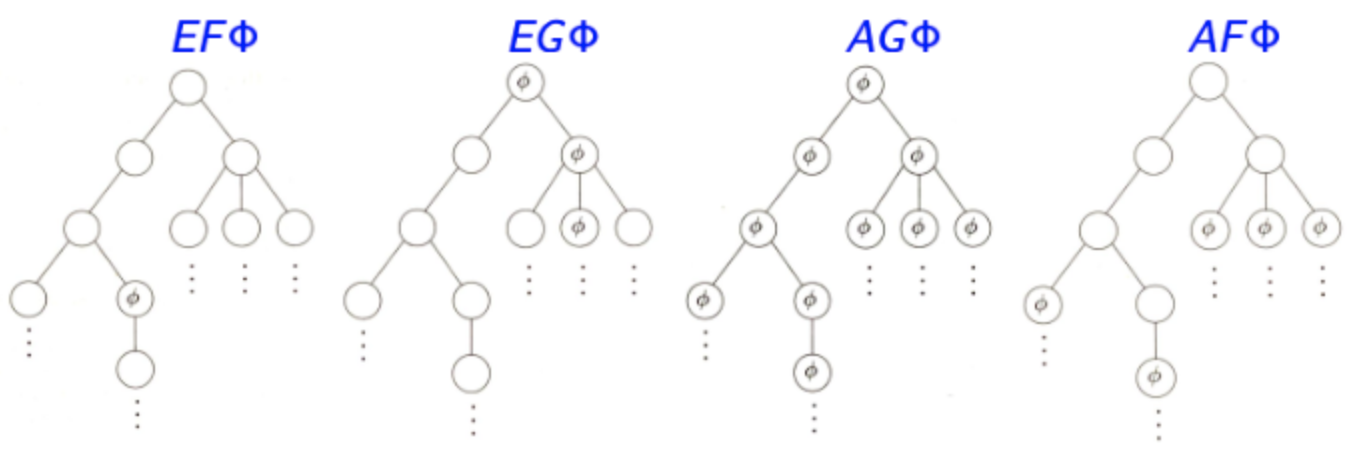
\includegraphics[width=\linewidth]{COMPSCI-2SD3/ctl.png}

\textbf{Equivalences}
$\neg AF\phi \equiv EG\neg\phi$\\
$\neg EF\phi \equiv AG\neg\phi$\\
$\neg AX\phi \equiv EX\neg\phi$\\
$AF\phi \equiv A[\top U \phi]$\\
$EF\phi \equiv E[\top I \phi]$

\subsubsection{Elevator Example 1}
``An upwards travelling elevator at the second floor does not change direction when it has passengers wishing to go to the fifth floor" \\
\textbf{CTL}: $AG(floor = 2 \land direction = up \land ButtonPressed5 \Rightarrow A[direction = up\ U\ floor = 5])$.\\
\subsubsection{Elevator Example 2}
``The elevator can remain idle on the third floor with its doors closed" \\
\textbf{CTL}: $AG((floor = 3 \land idle \land door = closed) \Rightarrow EG(floor = 3 \land idle \land door = closed))$

\subsection{LTL}
$\bot$ - false, $\top$ - true
Other symbols mean the same as above.
A set of paths satisfies $\phi$ if every path in the set satisfies $\phi$

\textbf{Equivalences}
$\neg G \phi \equiv F \neg \phi$ \\
$\neg F \phi \equiv G \neg \phi$ \\
$\neg X \phi \equiv X \neg \phi$ \\
$F(\phi \lor \psi) \equiv F\phi \lor F\psi$ \\
$G(\phi \land \psi) \equiv G\phi \land G\psi$ \\
$F\phi \equiv \top U \phi$ \\
$G\phi \equiv \bot R \phi$ \\
$\phi U \psi \equiv \phi W \psi \land F \psi$ \\
$\phi W \psi \equiv \phi U \psi \lor G \phi$ \\
$\phi W \psi \equiv \psi R(\phi \lor \psi)$ \\
$\phi R \psi \equiv \psi W(\phi \land \psi)$

\section{Dynamic Systems}
\subsection{Golf Club Program}
Players at a golf club borrow and then return golf balls. Different players need different numbers of balls. How do we model the infinite stream of players? We can only model infinite behaviours.
% Is there an example associated with this?

\subsection{Adverse Scheduling}
Intentionally schedule priorities to try to break things

Eg for golf club scheduling:
\begin{lstlisting}
progress NOVICE = {NOVICES.get[R]}
progress EXPERT = {EXPERTS.get[R]}
||ProgressCheck = GOLFCLUB >> {Players.put[R]}.
\end{lstlisting}

% todo: add master-slave stuff
\section{Q7 - A1}
\begin{lstlisting}
P = (a -> b -> d -> P).
Q = (c -> b -> e -> Q).
||S1 = (P || Q).

S2 = (a -> S2A | c -> S2B),
S2A = (c -> b -> d -> S2C | c -> b -> e -> S2D),
S2B = (a -> b -> d -> S2C | a -> b -> e -> S2D),
S2C = (e -> S2 | a -> e -> S2A),
S2D = (d -> S2 | c -> d -> S2B).
\end{lstlisting}
For the above FSPs, they both share the same LTS diagram (LTS version of the right petri net), however, since $||$S1 has simultaneous actions, its petri net will be show simultaneity whereas S2 will not. 
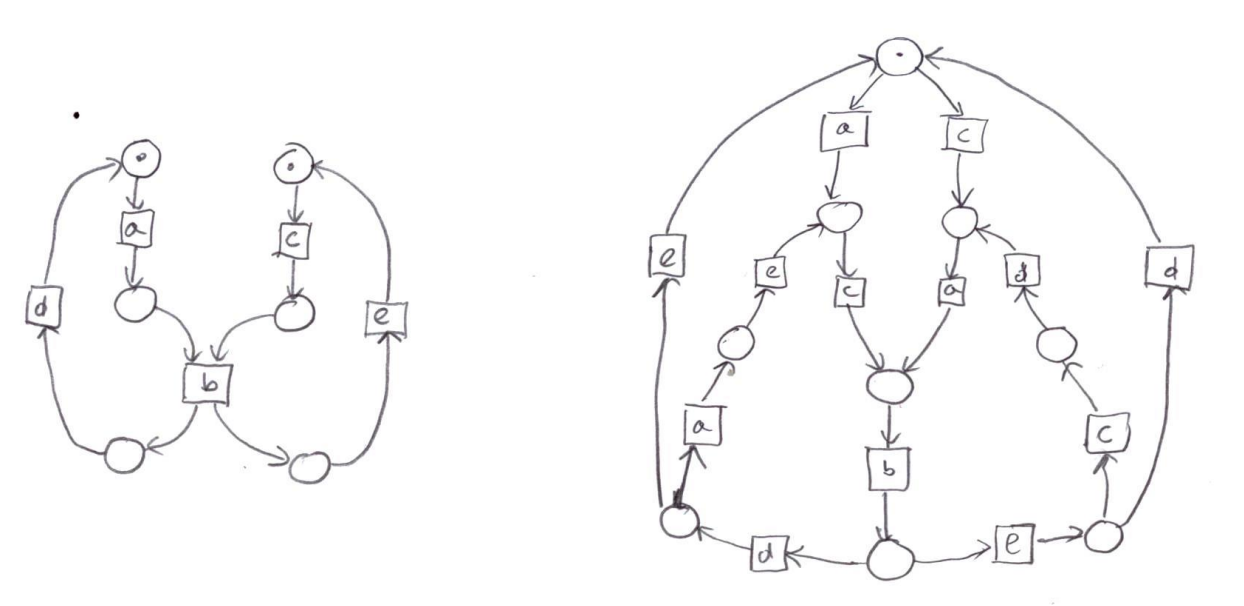
\includegraphics[width=\linewidth]{COMPSCI-2SD3/A1Q7.png}

\section{Q5 - Midterm}
A central computer is connected to remote terminals, with seats for concert hall. Clients choose a free seat and clerk enters the seat into the system and gives a ticket. We need to prevent double booking while letting clients choose any available seat.
\begin{lstlisting}
const False = 0
const True = 1
range Bool = False..True

SEAT = SEAT[False],
SEAT[reserved:Bool]
    = ( reserve -> SEAT[True]
      | query[reserved] -> SEAT[reserved]
      | when (reserved) reserve -> ERROR // error of reserved twice
      ).

range Seats = 0..1
||SEATS = (seat[Seats]:SEAT).

LOCK = (acquire -> release -> LOCK).

TERMINAL = (choose[s:Seats] -> acquire
            -> seat[s].query[reserved:Bool]
            -> (when(!reserved)seat[s].reserve -> release -> TERMINAL
            | when(reserved) release -> TERMINAL)
            ).

set Terminals = {a, b}
||CONCERT = (Terminals:TERMINAL || Terminals::SEATS || Terminals::LOCK).
\end{lstlisting}

\section{Q7 - Midterm}
\begin{lstlisting}
P1 = (a -> b -> c -> P1 | a -> c -> b -> P1).
P2 = (a -> (b -> c -> P2 | c -> b -> P2)).
Q = (b -> c -> Q).

||P1Q = (P1 || Q).
||P2Q = (P2 || Q).
\end{lstlisting}
For P1 there are two possible paths which have an $a$ transition. For P2, it starts with one $a$ transition, so both the starting states are equivalent in this case. In both branches of P1, you either do $b \rightarrow c \rightarrow P1$  or $c \rightarrow b \rightarrow P1$. For P2, it splits into two possible paths, $b \rightarrow c \rightarrow P2$ or $c \rightarrow b \rightarrow P2$, which is the same as the traces for P1. Therefore P1 and P2 are equivalent. \\
For $||$P1Q and $||$P2Q,both P1 and Q, and P2 and Q, share $b \rightarrow c$. In P1 and Q, this becomes a shared action and both P1 and Q will want to use the same transitions at the same time (deadlock). For $||$P2Q, the FSP can choose to go in the alternate direction instead of waiting for Q to finish, so this one would not have a deadlock whereas $||$P1Q will have one.
% add an image if we have space

\section{Alphabet Extension}
\subsection{Processes}
\begin{lstlisting}
P = (a -> b -> P).
Q = (c -> d -> Q).
Qa = (c -> d -> Q) + {b}.
\end{lstlisting}
When taking the composition of $||$PQ and $||$PQa, we take the union of both processes and remove duplicate transitions. In the case of PQ, there are no similar transitions, however PQa shares the b transition, so that is removed from the LTS.
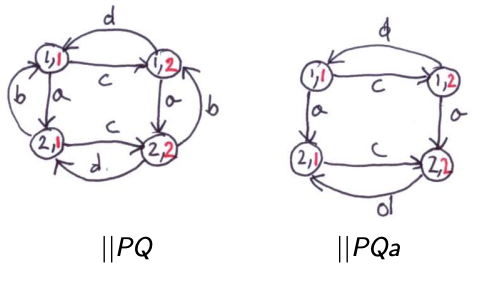
\includegraphics[width=\linewidth]{COMPSCI-2SD3/aep.png}

\subsection{Properties}
With properties, whenever you add more transitions through alphabet extension, you need to apply this transition to every state and use it as a transition to an error state.
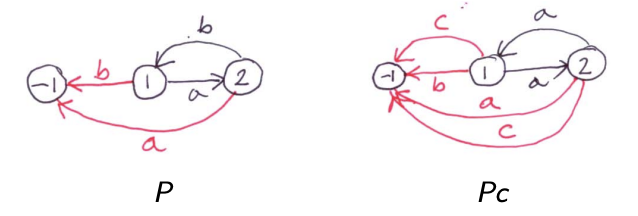
\includegraphics[width=\linewidth]{COMPSCI-2SD3/aep2.png}

% 
\includegraphics[width=\linewidth]{COMPSCI-2SD3/kita.png}

\section{Tut 6 Mutex Example}
Workers in an office share a printer. The printer is able to print any number of jobs before it runs out of toner. This is replaced by a technician when necessary.
\begin{lstlisting}
const J=3
range Jobs = 0..J
// j Represents toner
PRINTER = PRINTER [3],
PRINTER[j: Jobs] = ( when j==0 replace_toner->PRINTER[J] 
|when j>0 print_job -> PRINTER[j-1]).
USER = (print_job->USER).
const M = 2
range Users = 0..M
||USERS = (forall[i:Users] user [i]:USER).
TECHNICIAN=(replace_toner->TECHNICIAN).
||OFFICE=(USERS||PRINTER||TECHNICIAN)
/{user[Users].print_job/print_job}.
\end{lstlisting}

% this question was on both the 2020 and 2021 exam - bani (credit to cgn for the answer)
% please be on the exam 
\section{Binary Semaphore Question}
In an operating system, a binary semaphore is used to control access to the console. The console is used by user and system processes. Write down a model with FSP for this system. Discuss when user processes may be denied access to the console.
\begin{lstlisting}
BSEMA = (up -> down -> BSEMA).
PROCESS = (console.up -> console.down -> PROCESS).
set Processes = {user[1..2],system[1..2]}
OS = (Processes:PROCESS || Processes::console:BSEMA)>>{user}.
\end{lstlisting}

% dining savages?
% should there be multiple savages - like savage[i:1..N]:SAVAGES
% idk i just copied the posted example, i gotta shower but ill take a look after - json
% ok each savage does the same thing, there's no asymmetry or deadlocking possible so not numbering them is fine - json
\section{Dining Savages}
The dining savages: A tribe of savages eats communal dinners from a large pot capable of holding M servings of stewed missionaries. When a savage wants to eat, he helps himself from the pot unless it is empty, in which case he waits until the cook refills the pot. If the pot is empty, the cook refills the pot with M servings. The behavior of the savages and the cook is described by
\begin{lstlisting}
SAVAGE = (get_serving->SAVAGE).
COOK = (fill_pot->COOK).
\end{lstlisting}
Model the behaviour of the pot and of the system as FSP processes.
\begin{lstlisting}
const M = 5
SAVAGE = (getserving -> SAVAGE).
COOK = (fillpot -> COOK).
POT = SERVINGS[0],
SERVINGS[i:0..M] = (when (i==0) fillpot -> SERVINGS[M] | when (i>0) getserving -> SERVINGS[i-1]).

||SAVAGES = (SAVAGE || COOK || POT).
\end{lstlisting}

\section{Simplified Multidimensional Semaphores}
The extended primitives edown and eup are atomic (indivisible) and each operates on a set of semaphore variables which must be initiated with non-negative integer value. edown(S1,...,Sn): if for all i, $1\leq i\leq n$, Si>0 then for all i, $1\leq i\leq n$, $S_i := S_i -1$ else block execution of calling processes eup(S1,...,Sn): if processes blocked on (S1,...,Sn) then awaken one of them else for all i, $1\leq i\leq n$, $S_i := S_i +1$
\begin{lstlisting}
SEM(N=INITIAL_VALUE = SEMA[N],
SEMA[v:Int] = (when (v<=Max) up -> SEMA[v+1] | when (v>0) down -> SEMA[v-1]).
SEMS1S2(INITIAL1=3, INITIAL2=3) = (S1:SEM(3) || S2:SEM(3))\{S1.S2.up/S1.up, S1.S2.up/S2.up, S1.S2.down/S1.down, S1.S2.down/S1.down}.
\end{lstlisting} % mindlessly copied from the discord, not sure if its actually correct (that last /S1.down HAS to be S2 instead, right?) - bani

\section{Two Warring Neighbours}
Model this algorithm for two neighbours n1 and n2. Specified the required safety properties for the field and check that it does indeed ensure mutually exclusive access. Specify the required progress properties for the neighbours such that they both get to pick berries given a fair scheduling strategy.
% first line until 9th line is removable if tight on space, it should be provided in the question - bani
\begin{lstlisting}
const False = 0
const True = 1
range Bool = False..True
set BoolActions = {setTrue, setFalse, [False], [True]}
BOOLVAR = VAL[False],
VAL[v:Bool] = (setTrue  -> VAL[True]
              |setFalse -> VAL[False]
              |[v]      -> VAL[v]
              ).
||FLAGS = (flag1:BOOLVAR || flag2:BOOLVAR).
NEIGHBOUR1 = (flag1.setTrue -> TEST),
TEST       = (flag2[b:Bool] ->
                if(b) then
                   (flag1.setFalse -> NEIGHBOUR1)
                else
                   (enter -> exit -> flag1.setFalse -> NEIGHBOUR1)
              )+{{flag1,flag2}.BoolActions}.
NEIGHBOUR2 = (flag2.setTrue -> TEST),
TEST       = (flag1[b:Bool] ->
                if(b) then
                   (flag2.setFalse -> NEIGHBOUR2)
else
(enter -> exit-> flag2.setFalse -> NEIGHBOUR2)
              )+{{flag1,flag2}.BoolActions}.
property SAFETY = (n1.enter -> n1.exit -> SAFETY | n2.enter -> n2.exit -> SAFETY).
||FIELD = (n1:NEIGHBOUR1 || n2:NEIGHBOUR2 || {n1,n2}::FLAGS || SAFETY).
progress ENTER1 = {n1.enter} 
progress ENTER2 = {n2.enter}
||GREEDY = FIELD<<{{n1,n2}.{flag1,flag2}.setTrue}.
\end{lstlisting}

% REVIEW: apparently this might not be correct???
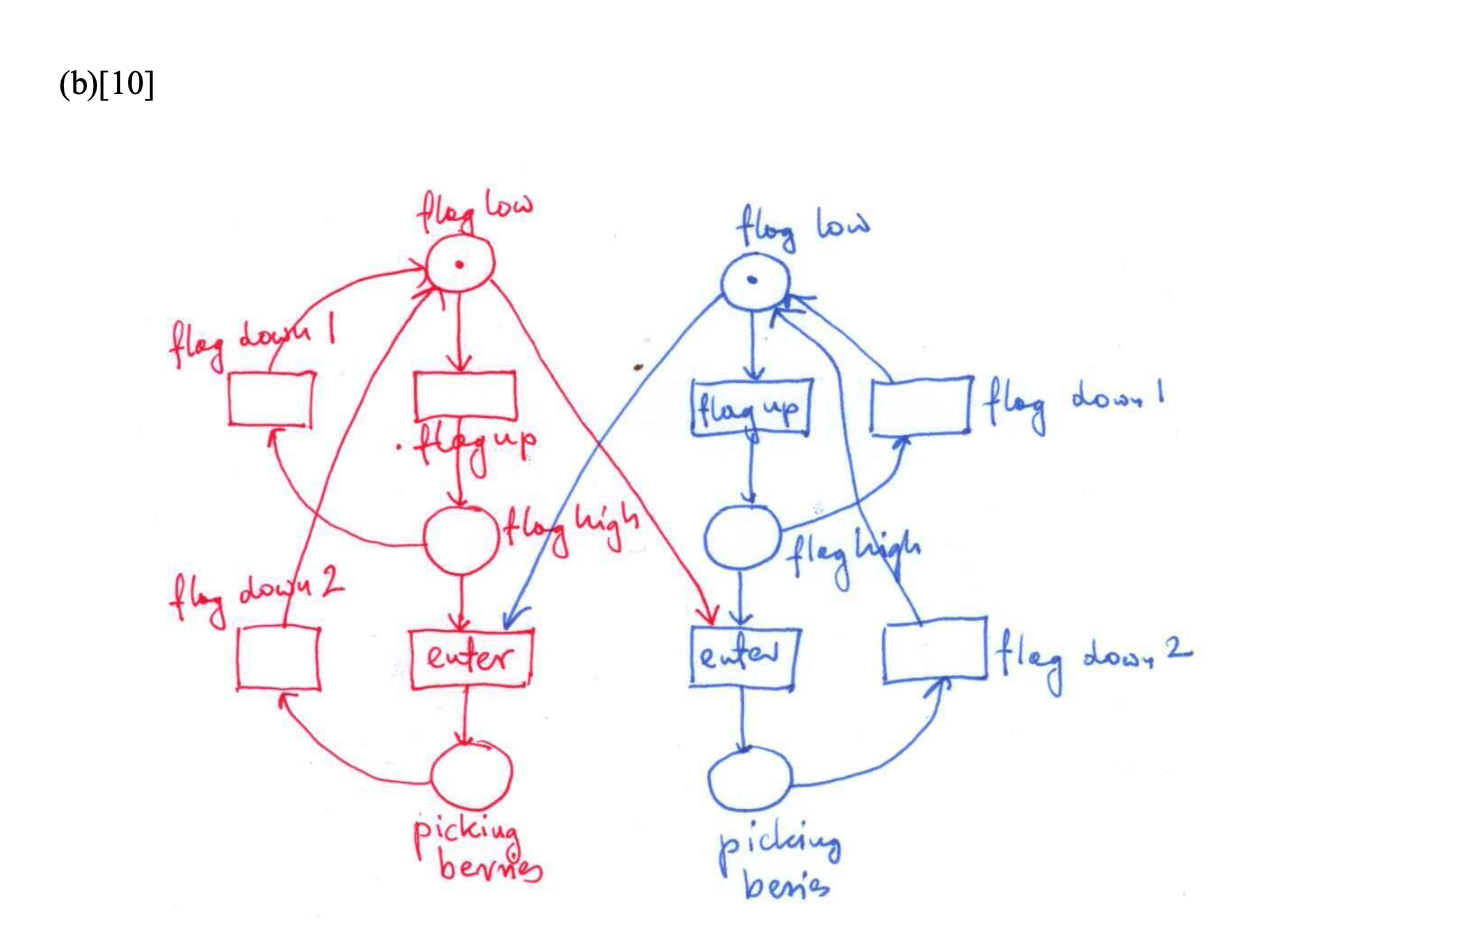
\includegraphics[width = \linewidth]{COMPSCI-2SD3/warring_neighbours_partb.png}

\section{CTL and LTL Examples}
% \begin{center}
%     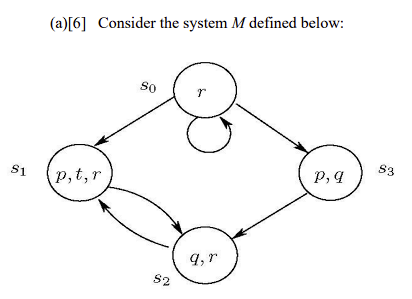
\includegraphics[width=.7\linewidth]{COMPSCI-2SD3/q8a.png}
% \end{center}
If the process is enabled infinitely often, then it runs infinitely often.
$$
\G\F enabled \Rightarrow \G\F running
$$
$$
\AG(\AF enabled) \Rightarrow \AG(\AF running)
$$

A passenger entering the elevator on 5th floor and pushing 2nd-floor button will never reach 6th floor, unless 6th-floor button is already lit or somebody will push it, no matter if she/he entered an upwards or upward travelling elevator.
% istg this question definition is just wrong
\begin{align*}
\AG(floor=5 \land ButtonPressed2 \Rightarrow \\
\A[\neg floor=6 \U ButtonPressed6])
\end{align*}

% was on A2 but just in case - bani
\section{Dining Philosophers with ‘atomic act of picking up both forks’}
\begin{lstlisting}
FORK = ( reserve_right -> take_right -> put_right -> FORK
| reserve_left -> take_left -> put_left -> FORK ).
PHIL = (think -> reserve_forks -> USE_FORKS).
USE_FORKS = ( take_right -> take_left -> eat -> PUT_FORKS
| take_left -> take_right -> eat -> PUT_FORKS ),
PUT_FORKS = ( put_left -> put_right -> PHIL
| put_right -> put_left -> PHIL ).
||DINERS(N=5) = ( forall[i:1..N]( phil[i]:PHIL || {phil[i].right,phil[(i+1)%N].left}::FORK) )
/{
reserve_forks/right.reserve_right,
reserve_forks/left.reserve_left,
reserve_forks_1/reserve_right_1,reserve_forks_1/reserve_left_2,
reserve_forks_2/reserve_right_2,reserve_forks_2/reserve_left_3,
reserve_forks_3/reserve_right_3,reserve_forks_3/reserve_left_4,
reserve_forks_4/reserve_right_4,reserve_forks_4/reserve_left_5,
reserve_forks_5/reserve_right_5,reserve_forks_5/reserve_left_1
}.
\end{lstlisting}

% we have extra space so:
\section{A3Q2 - Gas Question}
\begin{lstlisting}
const N = 3 //number of customers
const M = 2 //number of pumps
range C = 1..N
range P = 1..M
range A = 1..2 //Amount of money or Gas
CUSTOMER = (prepay[a:A]->gas[x:A]->
if (x==a) then CUSTOMER else ERROR).
CASHIER = (customer[c:C].prepay[x:A]->start[P][c][x]->CASHIER).
PUMP = (start[c:C][x:A] -> gas[c][x]->PUMP).
DELIVER = (gas[P][c:C][x:A]->customer[c].gas[x]->DELIVER).
||STATION = (CASHIER || pump[1..M]:PUMP || DELIVER)
/{pump[i:1..M].start/start[i],
pump[i:1..M].gas/gas[i]}.
||GASSTATION = (customer[1..N]:CUSTOMER ||STATION).
// part b
range T = 1..2
property FIFO = (customer[i:T].prepay[A] -> PAID[i]),
PAID[i:T] = (customer[i].gas[A] -> FIFO
|customer[j:T].prepay[A] -> PAID[i][j]),
PAID[i:T][j:T]= (customer[i].gas[A] -> PAID[j]).
||CHECK_FIFO = (GASSTATION || FIFO).
\end{lstlisting}

\section{A3Q3 - Cheese Question}
\begin{lstlisting}
set Bold = {bold[1..2]}
set Meek = {meek[1..2]}
set Customers = {Bold,Meek}
CUSTOMER = (getcheese->CUSTOMER).
COUNTER = (getcheese->COUNTER).
||CHEESE_COUNTER = (Customers:CUSTOMER || Customers::COUNTER).
\end{lstlisting}
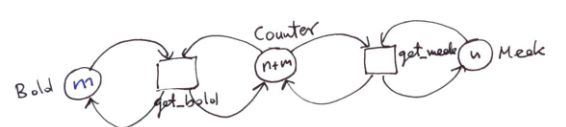
\includegraphics[width = \linewidth]{COMPSCI-2SD3/a3q3.png}

\section{Burger}
A cook puts burgers in a pot. A client checks if there is at least one burger in the pot, and if so, the client must take one.

Trace to error: fill[2], c2.check, fill[1], c1.check, c2.get, c1.get. Part b change pot to be:
\begin{lstlisting}
POT = POT[0]
POT[p: Burgers] = (when (p>0) check -> get -> POT[p-1] | fill[n: Burgers] -> POT[n]).
\end{lstlisting}
% i would add petri net but idt mine is right 

\end{multicols*}
\end{document}
